\def \secname {Stochastic (random) methods}

\section[\secname]{\hyperlink{toc}{\secname}}



\subsection{Overview}

Motivation

\begin{itemize}
    \item Many problems in physics have a non-deterministic or random or stochastic character

    \item Canonical example: Brownian motion; random walk - dynamics of particle subject to some random force

    \item Many other examples: includes almost all statistical mechanical systems

    \item Simulation is often impeded by the need to compute (accurate) expectation values of physical quantities

    \item Consider random walk

    \[ r^2(t^n) \rightarrow \langle r(t^n) \rangle\]

    where $\langle \ldots \rangle$ is average over \textbf{many} trials

    \item sometimes qualitative info can be extracted from small number of simulations
\end{itemize}

Coverage

\begin{itemize}
    \item Uniform random number generators (RNGs)
    \item Non-uniform random number generators
    \item Applications
    \begin{itemize}
        \item Diffusion limited Aggregation
        \item Ising Model
    \end{itemize}
\end{itemize}

\subsection{Pseudo-Random Number Generation (uniform)}

\begin{itemize}
    \item Almost all RNG in computer languages are algorithmic (deterministic); hence terminology `pseudo' RNG (PRNG)

    \item A PRNG can be characterized by a probability distribution function (PDF), p(x) such that 

    \[ p(x) dx \Rightarrow \text{probability that randomly generated number lies in internal x to x+dx}\]

    \item p(x) must be normalized on domain of interest $[x_{min}, x_{max}]$

    \[ \int_{x_{min}}^{x_{max}} p(x) dx = 1\]

    \item Caveat: floating point world is not the continuum, but we are going to ignore that point

    \item p(x) for uniform PRNG

    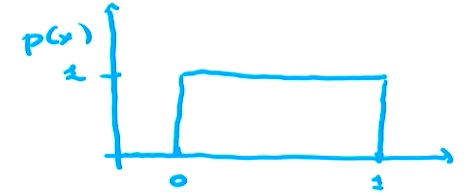
\includegraphics[width = 0.4 \linewidth]{Images/pdf_uniform.png}

    \item Many PRNG algorithms have been developed 

    \item MATLAB provides 9; see held for rng

    \item One common choice, \textbf{Linear Congruential Generator}

    \item Generates sequences of integers whose bit pattern can be interpreted as reals in the range [0,1]

    \[I_{n+1} = (aI_n + c) \text{mod}m\]

    where a and c are other integers and m is an integer called modulus

    \item Good choices for a,c will give maximal period m
\end{itemize}

Seeding a PRNG

\begin{itemize}
    \item MATLAB by design, will return same random number at start-up

    \item Change this behaviour by seeding the RNG. Forces the RNG to start somewhere else in it's sequence

    \item MATLAB

    \begin{verbatim}
        rng(seed)

        % where seed is a non-negative integer
        % same sequence always generated for same seed
    \end{verbatim}
\end{itemize}

\subsection{Pseudo-Random Number Generation (non-uniform)}

\begin{itemize}
    \item Consider some variable (deviate) which is randomly but not necessarily uniformly distributed in some interval $x_{\text{min}} \le x \le x_{\text{max}}$

    Examlpe: Gaussian Distibution ($-\infty < x < \infty$)


    \[ \text{PDF: } p(x) = \frac{1}{\sqrt{\pi \sigma}}e^{-x^2/\sigma^2}\]

    \item Many other examples: poisson, Maxwellian, ...

    \item Given $p(x)$, $x_{\text{min}}$, $x_{\text{max}}$ and a [0,...1] uniform PRNG such as MATLAB's rand, how can we generate deviates distributed according to $p(x)$?

    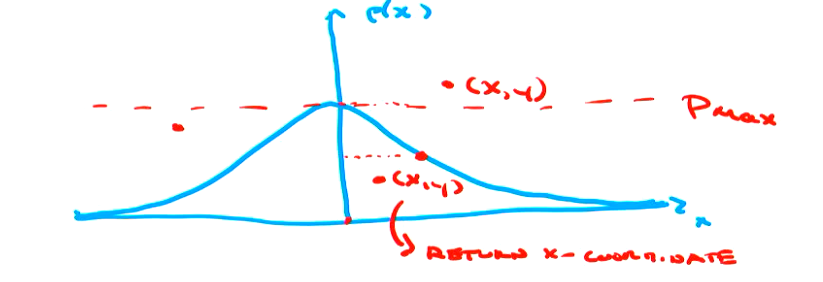
\includegraphics[width = 0.6 \linewidth]{Images/non_uniform_PRNG.png}

    \item Generate random points (x,y) [both coordinates randomly generated] in the region

    \[ x_{\text{min}} \le x \le x_{\text{max}} \]

    \[ y \le p_{\text{max}}\]

    \[ p_{\text{max}} = max(p(x))\]

    $\Rightarrow$ Rejects points that lie above $p(x)$, accepts points below p(x), returning $x$ as the deviate 

    \item Pseudo code for non-uniform PRNG

    \begin{verbatim}
    accept = false
    until accept do
        x = random(xmin, xmax)
        y = random(0,ymax)
        if y<p(x) then rand = x 
        accept = true
        end if
    end do
    \end{verbatim}

    Testing Implementation

    \item Generate large number, n, of deviates on [xmin, xmax]

    \item Compute approximation of PDF p(x) by ``binning" deviates; i.e. count number of deviates in each interval/bin

    \[ x_i \text{ to } x_i+\Delta x\]

    \[ x_1 = x_{\text{min}}\]

    \[ x_N = x_{\text{max}}\]

    \[ \Delta x = \frac{x_{\text{max}}-x_{\text{min}}}{N_1}\]

    \[ N-1 = \text{ \# of bins}\]

    \item Normalization (verify) let $c_i$ be the count for the i-th bin, then

    \[ \bar{c}_i = \frac{c_i}{n\Delta x}\]

    And 

    \[ lim_{n\rightarrow \infty , N \rightarrow \infty} \bar{c}_i = p(x_i)\]
    
\end{itemize}

\subsection{Diffusion Limited Aggregation (DLA)}

Model for growth of clusters $\Rightarrow$ collections of identical particles

Examples:

\begin{enumerate}
    \item Snow Flakes
    \item Soot particles
    \item Frost (Hoar Frost)
    \item Lightning; sparks
    \item Urban growth
\end{enumerate}

\begin{itemize}
    \item These clusters (aggregates) are characterized by dendritic (branching) structure

    \item Typically have non-integer dimensionality (fractal)

    \[ m(r) = \text{mass contained within radius r}\]

    \[ m(r) = r^d \rightarrow \text{fractal dimension}\]

    \[ \text{Typically} \quad 1 < d < 2\]
\end{itemize}

DLA Algorithm 

\begin{itemize}
    \item Use 2-D uniform lattice in (x,y)

    Particles: unit mass; two types

    \begin{itemize}
        \item Fixed/ Frozen: structure at some specific lattice site
        \item Mobile: free to random walk on lattice
    \end{itemize}

    Discrete time steps $t^n$

    Simplest Implementation

    \begin{itemize}
        \item One free particle at any time
        \item Particle random walks until becomes adjacent to a lattice site with fixed particle
        \item Free particle gets frozen at current position
        \item New random walker is launched
        \item Cluster: all fixed particles
    \end{itemize}

    Growth is \textbf{SLOW}

    \[ D_{\text{RMS}} = \langle D^2 \rangle^{\frac{1}{2}} \tilde n^\frac{1}{2}\]

    where n is the number of steps

    Extension: central bias

    \[ 0 \le b \le 1\]

    \[ b: \text{ Probability that walker takes extra step directly toward the center}\]

    \item Using the bias we can speed up the computation but it makes the fractal more clumpy and concentrated at the center. 
\end{itemize}

\textbf{missed friday class}



\textbf{November 27th 2023 11:06am (caught up)}

Recall: Monte Carlo Method (ISING system)

\begin{verbatim}
    if E_flip <= 0
        flip spin
    else 
        generate r = random(0,1)
        if re = exp(-E-flip((kBT)))
            flip spin
        else 
            leave spin as is
        end
    end
\end{verbatim}

\[ \Rightarrow \frac{P_1}{P_2} = \exp[-(E_1-E_2)/(k_BT)]\]

$\Rightarrow$ what is needed for thermal equilibrium?

\subsection{Physical Behaviour of Model}

\begin{itemize}
    \item System characterized by \textbf{competition}
    \begin{itemize}
        \item Ferromagnetic interaction tends to \textbf{order} system (spin alignment favoured as $T\rightarrow0$)
        \item Temperature tends to disorder system (spin completely randomized at high T)
    \end{itemize}
    \item At some critical temperature ($T_c$) and in the thermodynamic limit ($N\rightarrow\infty$) there will be a phase transition
\end{itemize}

Physical Quantities to measure (expectation values)

\begin{itemize}
    \item When simulating, need to give system time to equilibrate; then run for long enough to generate ``good statistics"
    \item Make passes through lattice; each pass generates new microstate $\alpha$; compute expectation values by averaging over these states
    \item Typically normalize quantities by dividing by number of spins
    \begin{itemize}
        \item Average energy $\langle E \rangle $
        \item Avergae magnetization $\langle M \rangle $
    \end{itemize}

    \[ E = - J \sum_{\langle ij\rangle} s_i s_j (-\mu H \sum_i s_i\]

    \item At T=0 (Take J=1); what is $\langle E \rangle$?

    \[ \langle E \rangle = -2J = -2; \]

    each spin contributes -4J;
    Divide by 2 to account for double-counting

    \item As $T\rightarrow \infty$, what is $\langle E \rangle$?

    \[ \langle E \rangle \rightarrow 0;\]
    But have to go to quite high T to see this since correlations among spins persist for even high T
\end{itemize}

Derived Quantities
\begin{itemize}
    \item Consider Variance of Energy

    \[ (\Delta E ) ^2 \equiv \langle E^2 \rangle - \langle E \rangle^2\]

    \item Fluctuation-Dissipation theorem (connects fluctuations to response of system to external perturbation). Relates to specific heat.

    \[ C = \frac{(\Delta E)^2}{k_B T^2}\]

    Will work in units where $k_B=1$

    \item Similarly, variance in M is related to susceptibility $\chi = \frac{dM}{dH}$ ($H\equiv$ Magnetic field)

    \[ \chi = \frac{(\Delta M)^2}{k_B T}\]

    Behaviour near $T=T_c$

    \item Scaling of Magnetization

    \[ M \sim (T-T_c)^{\beta}\]

    $\beta \rightarrow$ universal exponent

    \begin{center}
        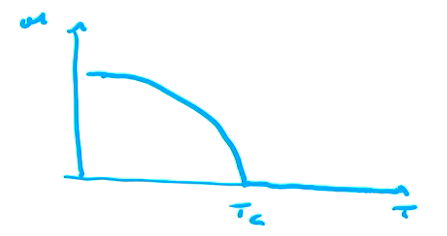
\includegraphics[width = 0.5\linewidth]{Images/ising_phase_transition.png}
    \end{center}

    \item exact solution of 2D ISING model (onsager 1944)

    \[ T_c = \frac{2}{ln(1+\sqrt{2}} = 2.2692 \ldots \]

    \[ \beta = \frac{1}{8}\]

    \item C and $\chi$ are divergent at $T=T_c$

    \item Phasee transition for $M=0$ is called second order or continuous since the order parameter $\langle M \rangle$ does not have a jump at $T=T_c$
    
\end{itemize}

\subsection{Behaviour of Model for $H\neq 0$}

\begin{itemize}
    \item Now have 2 extensive parameters: T, H

    \item Phase Diagram

    \begin{itemize}
        \item For low T, $T<T_c$, per spin magnetization is $<0$ on one side and $>0$ on other
    \end{itemize}

    \begin{center}
        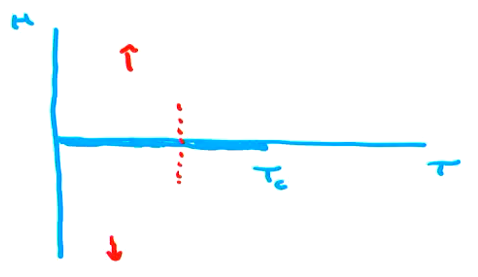
\includegraphics[width = 0.5\linewidth]{Images/H0_ising.png}
    \end{center}

    \item Thus, have a discontinuity in $\langle M \rangle $ as we tune across H=0
    \begin{center}
        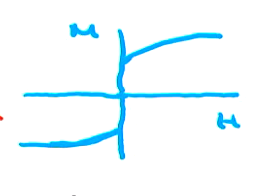
\includegraphics[width = 0.5\linewidth]{Images/MH_ising.png}
    \end{center}

    \item $\Rightarrow$ first order phase transition 
    \item Line in T-H plane 
    \item Above $T_c$ there is no spontaneous magnetization so no possibility of discontinuity in $\langle M \rangle$ as H passes through 0
    
    \item Phase transition line terminates at critical point

    $\Rightarrow$ general feature of first-order phase transition
    
\end{itemize}


\subsection{Phase Transitions}

\begin{center}
    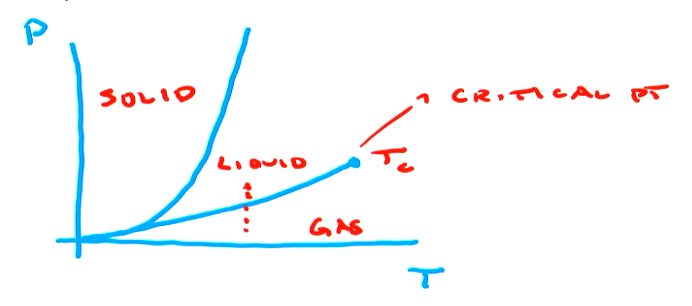
\includegraphics[width = 0.5\linewidth]{Images/phase_transtion_PT.png}
\end{center}

\begin{itemize}
    \item Similar situation: Gas-Liquid System: First order over a range of pressures, with a discontinuity in density
    \item As P increase, size of discontinuity decreases, vanishes at critical point
    \item Key difference between second order, first order phase transitions
    \begin{itemize}
        \item Second order: fluctuations become large near transition.
        \item First order: No growth in fluctuation near transition; happens suddenly
    \end{itemize}

    \item $\langle M \rangle $ vs H for ISING system can exhibit hysteresis, especially at low T
\end{itemize}
